\chapter{\abbr{pol3} \abbr{chip}-sequencing quantifies \abbr{trna} gene
expression}

\section{Quantifying expression of \trna genes}

We quantified \trna gene expression via \pol3 \chipseq. The reason for using
this, on the first glance indirect, measure is caused by the fact that \trna
genes are unfortunately not identifiable by their sequence alone: performing a
multiple sequence alignment of \trna genes in \mmu reveals that several \trna
genes share the exact same sequence.

\textfloat{trna-alignment}{spill}
    {\footnotesize\begingroup
\let\m\mismatch
\begin{tabular}{@{}ll@{}}
    \toprule
    chr5.trna1044 &  \seq{GTCTCTGTGGCGCAATCGGTtAGCGCGTTCGGCTGTTAACCGAAAG...........GtTGGTGGTTCGAGCCCACCCAGGGACG}\\
    chr3.trna750 &   \seq{GTCTCTGTGGCGCAATCGGTtAGCGCGTTCGGCTGTTAACCGAAAG...........GtTGGTGGTTCGAGCCCACCCAGGGACG}\\
    chr3.trna298 &   \seq{GTCTCTGTGGCGCAATCGGTtAGCGCGTTCGGCTGTTAACCGAAAG...........GtTGGTGGTTCGAGCCCACCCAGGGACG}\\
    chr3.trna294 &   \seq{GTCTCTGTGGCGCAATCGGTtAGCGCGTTCGGCTGTTAACCGAAAG...........GtTGGTGGTTCGAGCCCACCCAGGGACG}\\
    chr3.trna289 &   \seq{GTCTCTGTGGCGCAATCGGTtAGCGCGTTCGGCTGTTAACCGAAAG...........GtTGGTGGTTCGAGCCCACCCAGGGACG}\\
    chr2.trna1947 &  \seq{GTCTCTGTGGCGCAATCGGTtAGCGCGTTCGGCTGTTAACCGAAAG...........GtTGGTGGTTCGAGCCCACCCAGGGACG}\\
    chr1.trna1014 &  \seq{GTCTCTGTGGCGCAATCGGTtAGCGCGTTCGGCTGTTAACCGAAAG...........GtTGGTGGTTCGAGCCCACCCAGGGACG}\\
    chr11.trna1446 & \seq{GTCTCTGTGGCGCAATCGGTtAGCGCGTTCGGCTGTTAACCGAAAG...........GtTGGTGGTTCGAGCCCACCCAGGGACG}\\
    chr10.trna390 &  \seq{GTCTCTGTGGCGCAATCGGTtAGCGCGTTCGGCTGTTAACCGAAAG...........GtTGGTGGTTCGAGCCCACCCAGGGACG}\\
    chr3.trna757 &   \seq{GTCTC\m CGTGGCGCAAT\m CGGT\m cAGCGCGTTCGGCTGTTAACCGAAAG...........GtTGGTGGTTCGAGCCCACCC\m GGGGACG}\\
    chr3.trna283 &   \seq{GTCTCTGTGGCGCAATTGGTtAGCGCGTTCGGCTGTTAACCGAAAG...........GtTGGTGGTTC\m AAGCCCACCCAGGGACG}\\
    \bottomrule
\end{tabular}
\endgroup

    \todo{Fix alignment of table}}
    {Alignment of Asn \trna genes.}
    {Parts of a multiple sequence alignment of \trna genes in \mmu generated
    with COVE\@. Shown are the \trna genes coding for Asn. Bases which differ
    from the consensus sequence are highlighted in red.}

In order to identify individual \trna genes and quantify their expression, we
therefore cannot resort to conventional \rnaseq: the \rna reads covering only
the transcribed gene region are indistinguishable.
\todo{Biological background of pol3 ChIP}

With the \pol3 \chipseq data, we do not have this problem: reads cover both the
transcribed sequence and the flanking regions of each gene
(\cref{fig:trna-pol3-binding-profile}).

\textfig{trna-pol3-binding-profile}{spill}{\textwidth}
    {\trna \pol3 \chip binding profile.}
    {The shaded, bell-shaped area shows an idealised binding profile of \chipseq
    data spanning the \trna gene with the A and B box highlighted, as well as
    its flanking regions upstream and downstream of the gene body. This overlap
    plays a role in identifying the individual gene.}

When mapping the reads, we therefore do not discard all non-uniquely mapping
reads.\footnote{We still discard reads which are likely \pcr duplicates, i.e.\
map to many locations; we more or less arbitrarily used the threshold of
\num{20} non-unique mapping locations} We thus end up with reads which have not
been assigned to a given \trna gene (\cref{fig:trna-pol3-map-ambiguous-reads}).
In order to assign these reads to \trna genes, we \emph{reallocated} reads after
mapping, using the number of uniquely mapping reads in \trna genes’ flanking
regions to determine the most likely origin
(\cref{fig:trna-pol3-map-ambiguous-reads}) \citep{Kutter:2011}.

Formally, let \(i\) be the \(i\)th \trna gene locus, and \(c_i\) be the count of
uniquely mapped reads in its flanking region (we used \SI{\pm100}{bp}). A
multi-mapping read \(r\), which maps to a set \(T\) of candidate \trna[s], can
be allocated to a target \trna gene \(i\) randomly with probability

\begin{equation}
    p_i = \begin{cases}
        c_i\left(\sum_{x \in T}c_x\right)^{-1} &
            \text{if \(\sum_{x \in T}c_x \neq 0\),} \\
        \vert T \rvert^{-1} & \text{otherwise.}
    \end{cases}
\end{equation}

\textfloat{trna-pol3-map-ambiguous-reads}{spill}{%
    \centering
    \begingroup
        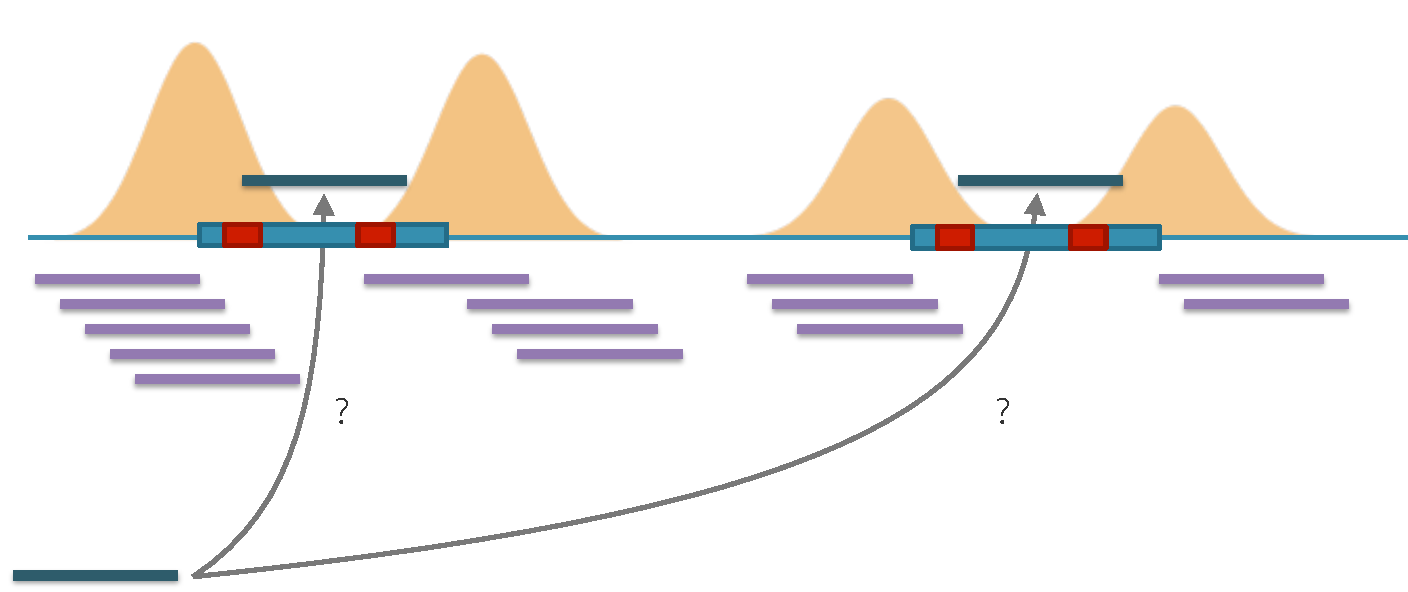
\includegraphics[width=\textwidth]{trna-pol3-map-ambiguous-reads-1}
        \subcaption{Two potential match candidate \trna genes for a read.}
    \endgroup
    \begingroup
        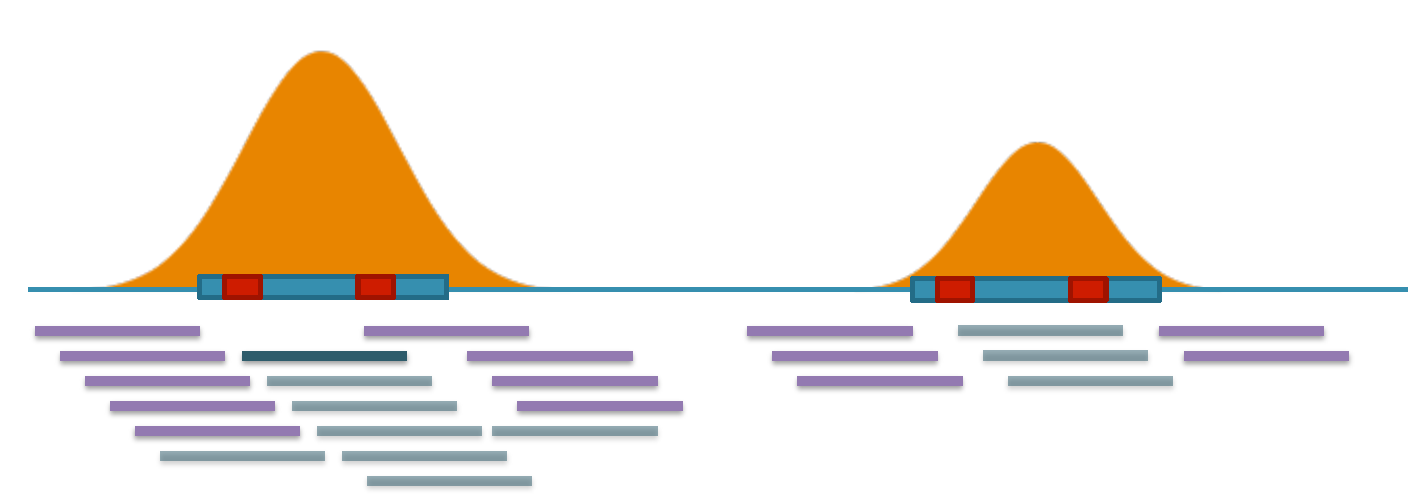
\includegraphics[width=\textwidth]{trna-pol3-map-ambiguous-reads-2}
        \subcaption{Using the count data from the flanking regions to
            extrapolate most likely mapping positions for ambiguous reads.}
    \endgroup}
    {Mapping ambiguous \chip reads.}
    {\chip reads originating from \trna genes can often not be mapped
    unambiguously to any given \trna. Instead, information form the gene’s
    flanking regions is used to determine the more likely provenance.}

Quantification of \trna genes was performed by first mapping the \pol3 \chipseq
data (non-strand-specific \SI{36}{bp} single-end reads sequenced by
\name{Illumina} \name{Genome Analyzer~IIx} or \name{HiSeq~2000}) using
\name{BWA} version 0.5.9-r16 \citep{Li:2009a} using default parameters. Next,
non-uniquely mapping reads were reallocated probabilistically according to the
description given above, using the \trna gene annotation from the \name{Genomic
\trna Database}, described in \citet{Chan:2009}. For each \trna gene (excluding
mitochondrial \trna genes), reads were summed on each \trna gene locus and in
the \SI{\pm100}{bp} flanking regions.

\trna genes that were unexpressed in all our experimental conditions were
excluded from the analysis, in order to reduce the effect of multiple testing,
and to exclude potential pseudogenes in the annotation. To be called expressed,
a \trna gene had to be present in all replicates of at least one condition with
a count of at least \num{10}, after size-factor normalisation. The threshold
\num{10} was chosen so that small variations in either direction would have a
minimal impact on the thresholding.
